\documentclass{mcmthesis}
\mcmsetup{CTeX = false,   % 使用 CTeX 套装时,设置为 true
        tcn = 2123481, problem =A,
        sheet = true, titleinsheet = true, keywordsinsheet = true,
        titlepage = true, abstract = true}
\usepackage{newtxtext}%\usepackage{palatino}
\usepackage{indentfirst}
\usepackage{float}
\title{The Fungi Decomposition Rate Model}
\author{Miao Fangran, Wang Xizhi, Wang Zhuo}
\date{\today}
\begin{document}
\begin{abstract}
  Question A of the Mathematical Modeling Competition of 2021 is A question about fungi. 
  Starting from fungi decomposition of landing plants, we are required to build A mathematical model to describe the decomposition of ground litter and wood fiber through fungal activities in the presence of a variety of fungi. 
  Provides model analysis and describes the interactions between different types of fungi. 
  This includes predictions of the relative strengths and weaknesses of each species and of combinations of species that are likely to persist. 
  Describe how the diversity of a fungal community within a system affects the overall efficiency of the system in decomposing litter on the ground.
  At the same time, we found many complex and effective and correct data, obtained our final mathematical formula through partial differential equations, and obtained models and images with tools such as MATLAB and Python, which were scientific and effective.
  The results clearly show that the decomposition rate of bacteria increases steadily at the beginning, and then after the density of species is saturated, the decomposition rate begins to decline rapidly.
\begin{keywords}
  Fungi; decomposition rate; MATLAB; python; Differential equation
\end{keywords}
\end{abstract}
\maketitle
%% Generate the Table of Contents, if it's needed.
\tableofcontents
\newpage
%%
%% Generate the Memorandum, if it's needed.
% \memoto{\LaTeX{}studio}
% \memofrom{Liam Huang}
% \memosubject{Happy \TeX{}ing!}
% \memodate{\today}
% % \logo{\LARGE I'm pretending to be a LOGO!}
% \begin{memo}[Memorandum]
% \end{memo}
%%
\section{Introduction}
\subsection{Problem Background}
Carbon cycle is a significant process in biosphere. 
It is the material circulation chain between the inorganic environment and organic organisms that keeps the balance of carbon dioxide in the atmosphere. 
The breakdown of organic material is a key component of the carbon cycle. 
It describes the exchange of carbon throughout the geochemical cycle, where the microorganisms play an important role. 
Fungi is a typical microorganism which is vital to decompose the plant material and woody fiber. 
It is significant to do meticulous study to fungus’ decomposition to the environment.

\subsection{Literature Review}
Fungal ecology is believed to play a crucial role in shaping Earth’s ecosystems because of fungi’s ability to recycle nutrients in the system as decomposers\cite{Fricker2017The}, provide resources as symbionts of the majority of land plants\cite{Treseder2015Fungal}, and impact the success and dynamics of other organisms as pathogens\cite{Smith2008Mycorrhizal,Maron2011Soil} 
It is significant to do meticulous study to fungus’ decomposition to the environment. 
By means of understanding the influence factor to the decomposition rate of the fungus thoroughly, scholar can apply it into other microorganism, and it has positive effect on ecosystem research. 
Recent research development have revealed that there are a considerable number of traits of fungi related to decomposition rate and certain traits link with each other\cite{Lustenhouwer11551}.
In that paper, several characters of fungi were discussed in order to determine the influence of wood decomposition. 
Researchers studied numerous traits associated with each fungus and tried to determine the role of these traits in wood block decomposition. 
In particular, the researchers found that are better able to adapt to different ranges of water conditions also tend to decompose wood more slowly. 
Fungi that grow faster and outperform other fungi tend to decompose wood faster\cite{Lustenhouwer11551}.

\subsection{Our work}
This paper will concentrate on two traits, the growth rate of fungus and the fungus’ tolerance to moisture. 
Based on statistic data of three fungi species, we match this data with a same form of formula by interpolation and matching, which can describe the relationship between the fungus’ growth rate, the fungus’ tolerance to moisture and the decomposition rate accurately with a certain range. 
Then this paper combines different species fungus together observe the composite effect of the decomposition to the ground litter. 
It assigns a value to fungus called “ranking”. 
This is the value to describe the competitive capacity of fungus, and we research the interaction between different species of fungus. 
To research how the fungus and environment have influence with each other, This paper introduces more variables with respect to the environment and revise the formula concerned with the decomposition rate. 
The effect of different environmental conditions on the decomposition rate of fungi were described more specifically. 
And the analysis of different species combination to the environment change indicates the importance of the biodiversity.
So this paper finally analyze the importance of the biodiversity to the whole environment when different degree of variations occur. 
It will make some sense in the field of ecology.


\section{Preparation of the Models}
\subsection{Assumptions}
Here are our assumptions:

For a single species of fungus\cite{Lustenhouwer11551}:
\begin{itemize}
  \item Under an ideal environment, which means that the temperature is perfect and the food is sufficient, the decomposition rate of fungi is mainly related to the extension rate and the moisture trade-off.
  \item The decomposition rate has a linear relationship with extension rate.
  \item The logarithm of decomposition rate has a linear relationship with moisture trade-off.
  \item If the environment is not so perfect, we introduce one parameter to adjust the decomposition rate---temperature.
\end{itemize}

With such condition, we can conclude two partial differential equations:
\begin{equation}
  \left\{
  \begin{aligned}
  &\frac{\partial f}{\partial x}&=C_1\\
  &\frac{\partial (\log f)}{\partial y}&=C_2
  \end{aligned}
  \right.
\end{equation}

Where $f$ represents the decomposition rate, $x$ represents extension rate and $y$ represents the moisture trade-off.
$C_1,C_2$ represents the linear slope between the independent variables and dependent variables.

Solve the equation, we acquire that:
\begin{equation}
  f=Ax\cdot e^{By}
\end{equation}
where $A$ and $B$ are constants, which varies with the type of fungi.

To adjust the decomposition rate with temperature, we introduce the Temperature function, which is $u(T)$.
Thus:
\begin{equation}
  f=u(T)\cdot Ax\cdot e^{By}
\end{equation}

When it comes to multiple fungi, we put forward our fifth assumption:
\begin{itemize}
  \item The decomposition rate will change when the number of fungus changes.
\end{itemize}
Then, we also introduce another function of one specific fungus' number:
\begin{equation}
  f=v(P)\cdot u(T)\cdot Ax\cdot e^{By}
\end{equation}

The last problem is that how to measure the decomposition rate.
Martin Witkamp\cite{10.2307/1933765} measured it by calculating the emission of carbon dioxide.
It reminded us of different measure method.
And what we need to do is to uniform the standard.
Thus, the last assumption is:
\begin{itemize}
  \item Every fungus decomposition rate can be measured by the amount of carbon dioxide released, and can also be translated into the mass loss of the raw material.
\end{itemize}
After that, we re-write $f$ in the form of $dm/dt$, where $m$ represents mass and $t$ represents time.

\subsection{Data Collection}
It is really hard to collect data for there are a lot of literature with different measurement indexes.
Thanks to the paper from Daniel et al.\cite{maynard2019consistent}, we get lots of useful data.
The relationship between fungi's decomposition rate and moisture niche width and the relationship between the decomposition rate and temperature.
Then uniform the standard---Express the rate of decomposition with the rate of mass loss.

Repeat such process with 5-6 papers, we finally get three fungi's data.

\begin{itemize}
  \item For fungus 1, $A=2.123,B=-0.4249$
  \item For fungus 2, $A=1.877,B=0.5152$
  \item For fungus 3, $A=3.553,B=0.7636$
\end{itemize}

For the correction factor, temperature and fungi's number, please check out in Appendix B for more information.
We created correction factors for each species.

\section{The Models}
To build up the model, we figure out that it is easy to use object-oriented programming.

We firstly set different objects for fungi.
The fungi itself have many attributes: the inherent coefficients $A$ and $B$, the extension rate, the decomposition rate, the number of fungi.
After setting the extension rate, we can get the decomposition rate and the number easily.

Then we set up the objects for environment:
The environment contains the following attributes: the moisture, temperature and wood number which represents the content of lignocellulosic.

After the interaction of the fungi and environment, we can get the curve of the rate of decomposition.

\subsection{Model 1}
In this model, we try to figure out the decomposition rate of one specific fungus against time under proper temperature. 
\begin{figure}[H]
  \centering
  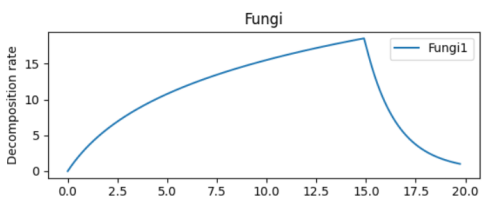
\includegraphics[width=0.8\textwidth]{figures/Model 1.png}
\end{figure}
We can conclude that the decomposition rate will increase as time goes on, for the number of fungus is increasing.
But when the number is too large, the content of lignocellulosic can't meet the fungus' requirement.
Then, the decomposition rate decreases.

\subsection{Model 2}
In this model, we try to figure out the interactions between the fungi.
\begin{figure}[H]
  \centering
  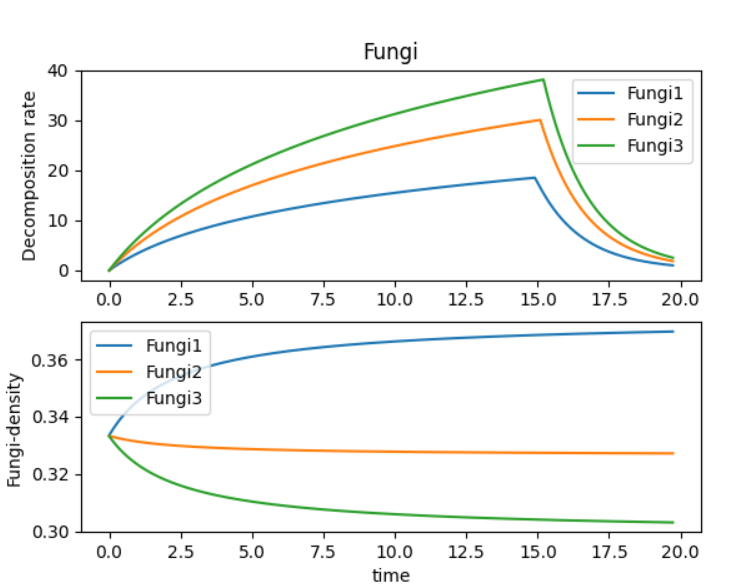
\includegraphics[width=0.8\textwidth]{figures/Model 2.png}
\end{figure}
We can conclude that almost all the fungi will experience the same process as model 1.
But the difference is that their density varies greatly.
Since in the competition within the population, one party may always become the dominant party, so that the number will occupy the majority.

\subsection{Model 3}
In this model, we try to figure out the interactions with the temperature.
\begin{figure}[H]
  \centering
  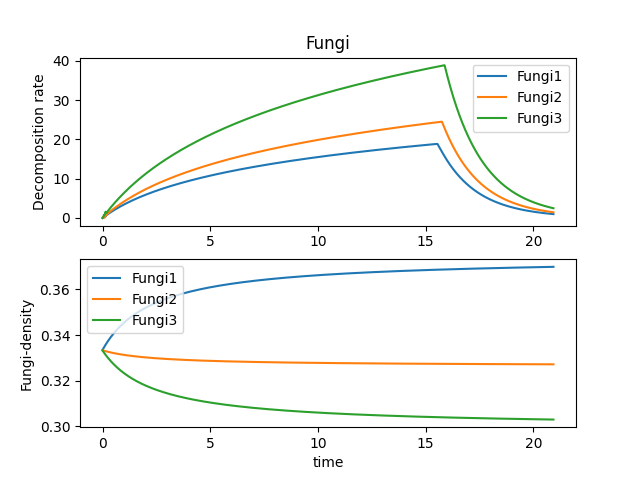
\includegraphics[width=0.8\textwidth]{figures/Model 3.png}
\end{figure}

We simulate the temperature from proper temperature to the low one and then to the high one.
We can still see that fungus 2's decomposition rate decrease obviously.
In the origin model, we set fungus 2 to be sensitive to the temperature while fungus 1 not.

\newpage
\subsection{Model 4}
In this model, we want to figure out the outside environment, such as dried, wet environment.
\begin{figure}[H]
  \centering
  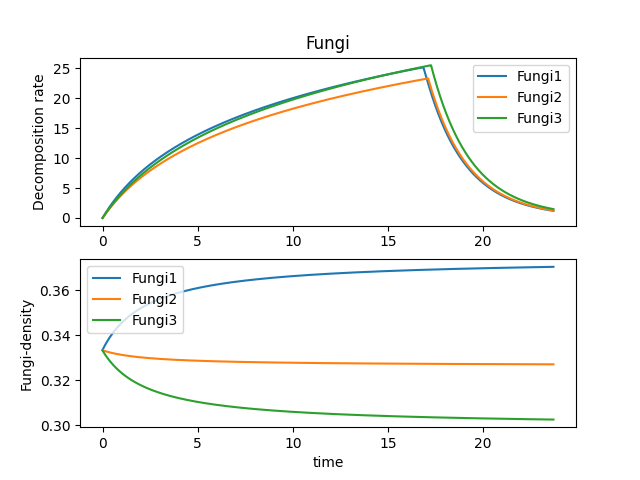
\includegraphics[width=0.6\textwidth]{figures/Model 4.png}
  \caption{The extremely dried environment}
\end{figure}

\begin{figure}[H]
  \centering
  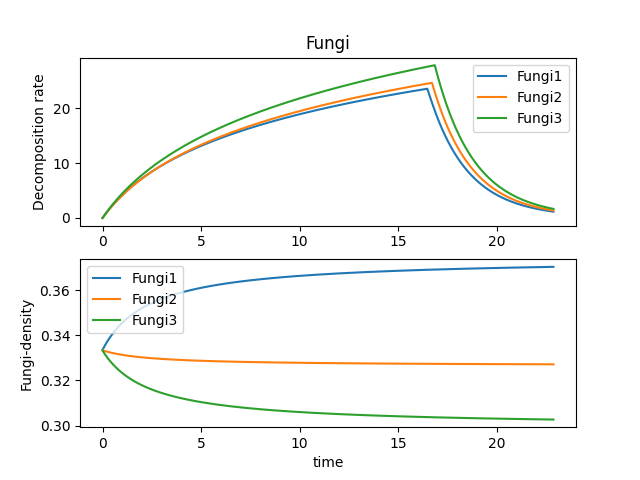
\includegraphics[width=0.6\textwidth]{figures/Model 5.png}
  \caption{The dried environment}
\end{figure}
The decomposition rates become the same as the environment get drier.
(Notice that the maximum of y-axis is 25)

\begin{figure}[H]
  \centering
  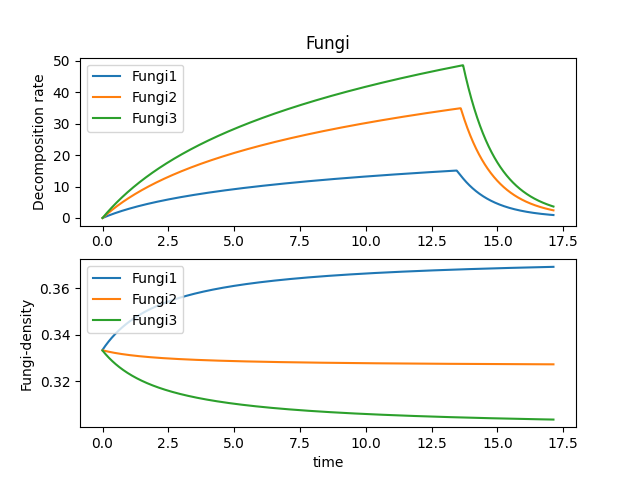
\includegraphics[width=0.6\textwidth]{figures/Model 6.png}
  \caption{The extremely wet environment}
\end{figure}

\begin{figure}[H]
  \centering
  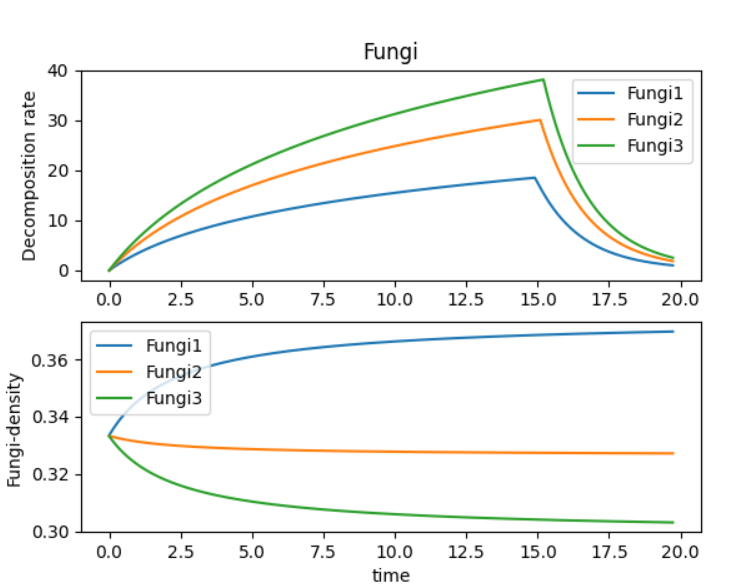
\includegraphics[width=0.6\textwidth]{figures/Model 2.png}
  \caption{The wet environment}
\end{figure}
The decomposition rate become higher as the environment get wetter.
(Notice that the maximum of y-axis is 50)

\section{Strengths and weaknesses}

\subsection{Strengths}
In this model, we set up two mutually related models, one is a single species, and the other is the community combination of multiple species.
Not only can we clearly see the change in the rate of decomposition of individual species.
There is also competition and dependence among multiple species, as well as changes in the rate of decomposition under community conditions.
We can also clearly see that the decomposition rate of bacteria increases steadily at the beginning, and then after the density of species is saturated, the decomposition rate begins to decline rapidly.

At the same time, we found many complex and effective and correct data, obtained our final mathematical formula through partial differential equations, and obtained models and images with tools such as MATLAB and Python, which were scientific and effective.


\subsection{Weaknesses}
\begin{itemize}
  \item We can't consider the death rate of each fungus, which means they grow in an almost ideal environment.
  \item The environment has lots of factors that can influence the decomposition rate of fungi, we just consider the moisture and the temperature.
  For instance, the light intensity can influence.
  \item We were only looking at fungi that break down carbon, however, there are also fungi can break down nitrogen.
  \item The shape of the colony may also affect the decomposition rate.
  \item We only consider the inner influence within the single population---fungi. We can't consider other living things' influence.
\end{itemize}

\medskip

\bibliographystyle{unsrt}
\bibliography{references}

\newpage

\begin{appendices}

\section{First appendix}


\newpage
\section{Second appendix}

% some more text \textcolor[rgb]{0.98,0.00,0.00}{\textbf{Input C++ source:}}
% \lstinputlisting[language=C++]{./code/mcmthesis-sudoku.cpp}
The class of \textcolor[rgb]{0.98,0,0}{\textbf{Fungi}} and \textcolor[rgb]{0.98,0,0}{\textbf{environment}} are as below:
\lstinputlisting[language=python]{./code/Fungi.py}

The \textcolor[rgb]{0.98,0,0}{\textbf{main code}} is as below:
\lstinputlisting[language=python]{./code/main.py}

\end{appendices}
\end{document}
